%% LyX 2.3.4.2 created this file.  For more info, see http://www.lyx.org/.
%% Do not edit unless you really know what you are doing.
\documentclass[english,dvipsnames,aspectratio=169]{beamer}
\usepackage{mathptmx}
\usepackage{eulervm}
\usepackage[T1]{fontenc}
\usepackage[latin9]{inputenc}
\usepackage{babel}
\usepackage{amstext}
\usepackage{amssymb}
\usepackage{graphicx}
\usepackage{ifthen}
\usepackage{xcolor}
\usepackage{xspace}
\usepackage{tikz}
\usetikzlibrary{tikzmark}
\usetikzlibrary{calc}
\usepackage{pgfplots}
%\pgfplotsset{compat=1.17}
\usepackage{booktabs}
\usepackage{xpatch}

\usepackage{pgfpages}
\setbeamertemplate{note page}{\pagecolor{yellow!5}\insertnote}
%\setbeameroption{hide notes} % Only slides
%\setbeameroption{show only notes} % Only notes
%\setbeameroption{show notes on second screen=right} % Both

%\usepackage{pdfcomment}
%\newcommand{\pdfnote}[1]{\marginnote{\pdfcomment[icon=note]{#1}}}
\newcommand{\pdfnote}[1]{}

\xpatchcmd{\itemize}
  {\def\makelabel}
  {\ifnum\@itemdepth=1\relax
     \setlength\itemsep{2ex}% separation for first level
   \else
     \ifnum\@itemdepth=2\relax
       \setlength\itemsep{1ex}% separation for second level
     \else
       \ifnum\@itemdepth=3\relax
         \setlength\itemsep{0.5ex}% separation for third level
   \fi\fi\fi\def\makelabel
  }
 {}
 {}

\ifx\hypersetup\undefined
  \AtBeginDocument{%
    \hypersetup{unicode=true,pdfusetitle,
 bookmarks=true,bookmarksnumbered=false,bookmarksopen=false,
 breaklinks=false,pdfborder={0 0 0},pdfborderstyle={},backref=false,colorlinks=true,
 allcolors=NYUPurple,urlcolor=LightPurple}
  }
\else
  \hypersetup{unicode=true,pdfusetitle,
 bookmarks=true,bookmarksnumbered=false,bookmarksopen=false,
 breaklinks=false,pdfborder={0 0 0},pdfborderstyle={},backref=false,colorlinks=true,
 allcolors=NYUPurple,urlcolor=LightPurple}
\fi

\makeatletter

%%%%%%%%%%%%%%%%%%%%%%%%%%%%%% LyX specific LaTeX commands.
%% Because html converters don't know tabularnewline
\providecommand{\tabularnewline}{\\}

%%%%%%%%%%%%%%%%%%%%%%%%%%%%%% Textclass specific LaTeX commands.
% this default might be overridden by plain title style
\newcommand\makebeamertitle{\frame{\maketitle}}%
% (ERT) argument for the TOC
\AtBeginDocument{%
  \let\origtableofcontents=\tableofcontents
  \def\tableofcontents{\@ifnextchar[{\origtableofcontents}{\gobbletableofcontents}}
  \def\gobbletableofcontents#1{\origtableofcontents}
}

%%%%%%%%%%%%%%%%%%%%%%%%%%%%%% User specified LaTeX commands.
\usetheme{CambridgeUS} 
\beamertemplatenavigationsymbolsempty


% Set Color ==============================
\definecolor{NYUPurple}{RGB}{87,6,140}
\definecolor{LightPurple}{RGB}{165,11,255}


\setbeamercolor{title}{fg=NYUPurple}
\setbeamercolor{frametitle}{fg=NYUPurple}

\setbeamercolor{background canvas}{fg=NYUPurple, bg=white}
\setbeamercolor{background}{fg=black, bg=NYUPurple}

\setbeamercolor{palette primary}{fg=black, bg=gray!30!white}
\setbeamercolor{palette secondary}{fg=black, bg=gray!20!white}
\setbeamercolor{palette tertiary}{fg=gray!20!white, bg=NYUPurple}

\setbeamertemplate{headline}{}
\setbeamerfont{itemize/enumerate body}{}
\setbeamerfont{itemize/enumerate subbody}{size=\normalsize}
\setbeamerfont{itemize/enumerate subsubbody}{size=\normalsize}

\setbeamercolor{parttitle}{fg=NYUPurple}
\setbeamercolor{sectiontitle}{fg=NYUPurple}
\setbeamercolor{sectionname}{fg=NYUPurple}
\setbeamercolor{section page}{fg=NYUPurple}
%\setbeamercolor{description item}{fg=NYUPurple}
%\setbeamercolor{block title}{fg=NYUPurple}

\setbeamertemplate{blocks}[rounded][shadow=false]
\setbeamercolor{block body}{bg=normal text.bg!90!NYUPurple}
\setbeamercolor{block title}{bg=NYUPurple!30, fg=NYUPurple}



\AtBeginSection[]{
  \begin{frame}
  \vfill
  \centering
\setbeamercolor{section title}{fg=NYUPurple}
 \begin{beamercolorbox}[sep=8pt,center,shadow=true,rounded=true]{title}
    \usebeamerfont{title}\usebeamercolor[fg]{title}\insertsectionhead\par%
  \end{beamercolorbox}
  \vfill
  \end{frame}
}

\makeatother

\setlength{\parskip}{\medskipamount} 

\input ../macros

\begin{document}
\input ../rosenberg-macros

\title[CSCI-GA 2565]{Kernel Methods}
\author{Mengye Ren}

\date{February 22, 2022}
\institute{CDS, NYU}

\makebeamertitle
\mode<article>{Just in article version}

\begin{frame}
    Logistics:\\
    \begin{itemize}
        \item Please fill out the course survey so that we can better help you
        \item Feel free to ask questions during the lab
    \end{itemize}

    Today's lecture:\\
    \begin{itemize}
        \item Wrap-up SVM
        \item Motivation of kernel methods: Our data is typically not linearly separable, but we like to work with linear models.
        \item Adding features (going to high-dimensional space) allow us to use linear models for complex data.
        \item Kernels allow us to think about similarities rather than feature engineering.
    \end{itemize}
\end{frame}

\section{Feature Maps}

\begin{frame}{The Input Space $\cx$}
\begin{itemize}
\item Our general learning theory setup: no assumptions about $\cx$

\item But $\cx=\reals^{d}$ for the specific methods we've developed: 
\begin{itemize}
\item Ridge regression
\item Lasso regression
\item Support Vector Machines 
\end{itemize}
\item Our hypothesis space for these was all affine functions on $\reals^{d}$:
\[
\cf=\left\{ x\mapsto w^{T}x+b\mid w\in\reals^{d},b\in\reals\right\} .
\]
\item What if we want to do prediction on inputs not natively in $\reals^{d}$?
\end{itemize}
\end{frame}
%
\begin{frame}{The Input Space $\cx$}
\begin{itemize}
\item Often want to use inputs not natively in $\reals^{d}$:
\begin{itemize}
\item Text documents
\item Image files
\item Sound recordings
\item DNA sequences
\end{itemize}

\item But everything in a computer is a sequence of numbers
\begin{itemize}
\item The $i$th entry of each sequence should have the same ``meaning''
\item All the sequences should have the same length
\end{itemize}
\end{itemize}
\end{frame}

\begin{frame}{Feature Extraction}
\begin{definition}
Mapping an input from $\cx$ to a vector in $\reals^{d}$ is called
\textbf{feature extraction} or \textbf{featurization}. 
\end{definition}

\begin{center}
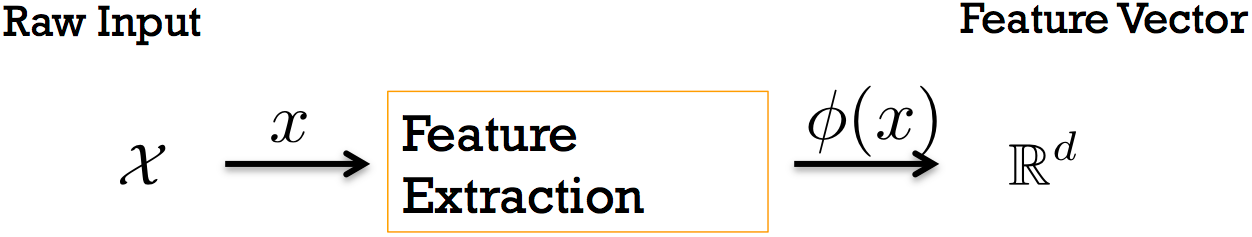
\includegraphics[width=0.9\textwidth]{figures/feature-extraction}
\par\end{center}

\end{frame}
%
\begin{frame}{Linear Models with Explicit Feature Map}
\begin{itemize}
\item Input space: $\cx$ (no assumptions)
\item Introduce \textbf{feature map} $\phi:\cx\to\reals^{d}$
\item The feature map maps into the \textbf{feature space} $\reals^{d}$.

\item Hypothesis space of affine functions on feature space:
\[
    \cf=\left\{ x\mapsto w^{T}{\color{blue}\phi(x)}+b\mid w\in\reals^{d},b\in\reals\right\} .
\]
\end{itemize}
\end{frame}
%
\begin{frame}{Geometric Example: Two class problem, nonlinear boundary}
\begin{center}
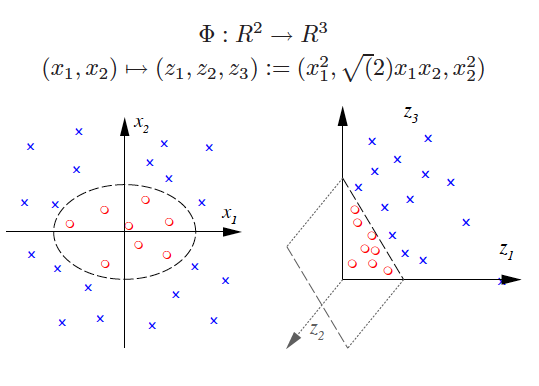
\includegraphics[height=0.6\textheight]{figures/feature-map-3d}
\par\end{center}
    \vspace{-1em}
\begin{itemize}
\item With identity feature map $\phi(x)=\left(x_{1},x_{2}\right)$ and
linear models, can't separate regions

\item With appropriate featurization $\phi(x)=\left(x_{1},x_{2},x_{1}^{2}+x_{2}^{2}\right)$,
becomes linearly separable . 

\item Video: \url{http://youtu.be/3liCbRZPrZA} 
\end{itemize}
    \let\thefootnote\relax\footnotetext{\tiny{\url{https://math.stackexchange.com/questions/353607/how-do-inner-product-space-determine-half-planes}}}
\end{frame}
%
\begin{frame}{Expressivity of Hypothesis Space}
\begin{itemize}
\item For linear models, to grow the hypothesis spaces, we must add features.

\item Sometimes we say a larger hypothesis is \hl{more expressive}. 
\begin{itemize}
\item (can fit more relationships between input and action)
\end{itemize}

\item Many ways to create new features.
\end{itemize}
\end{frame}
%

\section{Handling Nonlinearity with Linear Methods}
\begin{frame}{Example Task: Predicting Health}
\begin{itemize}
\item General Philosophy: Extract every feature that might be relevant

\item Features for medical diagnosis
\begin{itemize}
\item height
\item weight
\item body temperature
\item blood pressure
\item etc...
\end{itemize}
\end{itemize}
\let\thefootnote\relax\footnotetext{\tiny{From Percy Liang's "Lecture 3" slides from Stanford's CS221, Autumn 2014. }}
\end{frame}

\begin{frame}{Feature Issues for Linear Predictors}
\begin{itemize}
\item For linear predictors, it's important \textbf{how} features are added
    \begin{itemize}
        \item The relation between a feature and the label may not be linear
        \item There may be complex dependence among features
    \end{itemize}

\item Three types of nonlinearities can cause problems:

\begin{itemize}
\item Non-monotonicity
\item Saturation
\item Interactions between features
\end{itemize}
\end{itemize}
\let\thefootnote\relax\footnotetext{\tiny{From Percy Liang's "Lecture 3" slides from Stanford's CS221, Autumn 2014. }}
\end{frame}

\begin{frame}{Non-monotonicity: The Issue}
\begin{itemize}
\item Feature Map: $\phi(x)=\left[1,\text{temperature}(x)\right]$

\item Action: Predict health score $y\in\reals$ (positive is good)

\item Hypothesis Space $\cf{=}\left\{ \mbox{affine functions of temperature}\right\} $

\item Issue: 

\begin{itemize}
\item Health is not an affine function of temperature.

\item Affine function can either say
\begin{itemize}
\item Very high is bad and very low is good, or
\item Very low is bad and very high is good,
\item But here, both extremes are bad.
\end{itemize}
\end{itemize}
\end{itemize}
\let\thefootnote\relax\footnotetext{\tiny{From Percy Liang's "Lecture 3" slides from Stanford's CS221, Autumn 2014. }}
\end{frame}

\begin{frame}{Non-monotonicity: Solution 1}
\begin{itemize}
\item Transform the input:
\[
\phi(x)=\left[1,\left\{ \text{temperature(x)-37}\right\} ^{2}\right],
\]
where $37$ is ``normal'' temperature in Celsius.

\item Ok, but requires manually-specified domain knowledge
\begin{itemize}
\item Do we really need that?
\item What does $w^T\phi(x)$ look like?
\end{itemize}
\end{itemize}
\let\thefootnote\relax\footnotetext{\tiny{From Percy Liang's "Lecture 3" slides from Stanford's CS221, Autumn 2014. }}
\end{frame}

\begin{frame}{Non-monotonicity: Solution 2}
\begin{itemize}
\item Think less, put in more:
\[
\phi(x)=\left[1,\text{temperature}(x),\left\{ \text{temperature}(x)\right\} ^{2}\right].
\]


\item \hl{More expressive} than Solution 1.

\end{itemize}
\begin{block}{General Rule}

Features should be simple building blocks that can be pieced together.
\end{block}
\let\thefootnote\relax\footnotetext{\tiny{From Percy Liang's "Lecture 3" slides from Stanford's CS221, Autumn 2014. }}
\end{frame}

\begin{frame}{Saturation: The Issue}
\begin{itemize}
\item Setting: Find products relevant to user's query

\item Input: Product $x$
\item Action: Score the relevance of $x$ to user's query

\item Feature Map:
\[
\phi(x)=\left[1,N(x)\right],
\]
where $N(x)=\text{number of people who bought }x$.

\item We expect a monotonic relationship between $N(x)$ and relevance,
    but also expect \hl{diminishing return}.
\end{itemize}
\let\thefootnote\relax\footnotetext{\tiny{From Percy Liang's "Lecture 3" slides from Stanford's CS221, Autumn 2014. }}
\end{frame}

\begin{frame}{Saturation: Solve with nonlinear transform}
\begin{itemize}
\item Smooth nonlinear transformation:
\[
\phi(x)=\left[1,\log\left\{ 1+N(x)\right\} \right]
\]

        \begin{itemize}
    \item $\log\left(\cdot\right)$ good for values with large dynamic ranges
    \end{itemize}
\item Discretization (a discontinuous transformation):
\[
\phi(x)=\left(\ind{0\le N(x)<10},\ind{10\le N(x)<100},\ldots\right)
\]

        \begin{itemize}
\item Small buckets allow quite flexible relationship
        \end{itemize}

\end{itemize}
\let\thefootnote\relax\footnotetext{\tiny{From Percy Liang's "Lecture 3" slides from Stanford's CS221, Autumn 2014. }}
\end{frame}

\begin{frame}{Interactions: The Issue}
\begin{itemize}
\item Input: Patient information $x$
\item Action: Health score $y\in\reals$ (higher is better)
\item Feature Map
\[
\phi(x)=\left[\mbox{height}(x),\mbox{weight}(x)\right]
\]


\item Issue: It's the weight \textit{relative} to the height that's important.

\item Impossible to get with these features and a linear classifier.
\item Need some \textbf{interaction} between height and weight.

\let\thefootnote\relax\footnotetext{\tiny{From Percy Liang's "Lecture 3" slides from Stanford's CS221, Autumn 2014. }}
\end{itemize}
\end{frame}

\begin{frame}{Interactions: Approach 1}
\begin{itemize}
\item Google ``ideal weight from height''

\item J. D. Robinson's ``ideal weight'' formula (for a male):
\[
\mbox{weight}\mbox{(kg)}=52+1.9\left[\mbox{height(in)}-60\right]
\]


\item Make score square deviation between height($h$) and ideal weight($w$)
\[
f(x)=\left(52+1.9\left[h(x)-60\right]-w(x)\right)^{2}
\]


\item WolframAlpha for complicated Mathematics:
\[
f(x)=3.61h(x)^{2}-3.8h(x)w(x)-235.6h(x)+w(x)^{2}+124w(x)+3844
\]
\end{itemize}
\let\thefootnote\relax\footnotetext{\tiny{From Percy Liang's "Lecture 3" slides from Stanford's CS221, Autumn 2014. }}
\end{frame}

\begin{frame}{Interactions: Approach 2}
\begin{itemize}
\item Just include all second order features:
\[
\phi(x)=\left[1,h(x),w(x),h(x)^{2},w(x)^{2},\underbrace{h(x)w(x)}_{\mbox{cross term}}\right]
\]

\item More flexible, no Google, no WolframAlpha.
\end{itemize}
\begin{block}{General Principle}

Simpler building blocks replace a single ``smart'' feature.
\end{block}
\let\thefootnote\relax\footnotetext{\tiny{From Percy Liang's "Lecture 3" slides from Stanford's CS221, Autumn 2014. }}
\end{frame}

%\begin{frame}{Predicate Features and Interaction Terms}
%\begin{definition}
%A \textbf{predicate} on the input space $\cx$ is a function $P:\cx\to\left\{ \mbox{True},\mbox{False}\right\} $.
%
%\pause{}
%\end{definition}
%
%\begin{itemize}
%\item Many features take this form:
%\begin{itemize}
%\item $x\mapsto s(x)=\ind{\mbox{subject is sleeping}}$
%\item $x\mapsto d(x)=\ind{\mbox{subject is driving}}$
%
%\pause{}
%\end{itemize}
%\item For predicates, interaction terms correspond to \textbf{AND} conjunctions:
%\begin{itemize}
%\item $x\mapsto s(x)d(x)=\ind{\mbox{subject is sleeping AND subject is driving}}$
%\end{itemize}
%\end{itemize}
%\let\thefootnote\relax\footnotetext{\tiny{From Percy Liang's "Lecture 3" slides from Stanford's CS221, Autumn 2014. }}
%\end{frame}

\begin{frame}{Monomial Interaction Terms}
    \textbf{Interaction terms} are useful building blocks to model non-linearities in features.
\begin{itemize}
\item Suppose we start with $x=\left(1,x_{1},\ldots,x_{d}\right)\in\reals^{d+1}=\cx$.

\item Consider adding all \textbf{monomials} of degree $M$: $x_{1}^{p_{1}}\cdots x_{d}^{p_{d}}$,
with $p_{1}+\cdots+p_{d}=M$.
        \begin{itemize}
            \item Monomials with degree 2 in 2D space: $x_1^2$, $x_2^2$, $x_1x_2$
        \end{itemize}
\item How many features will we end up with? ${M+d-1 \choose M}$ (``stars and bars'')
    \pdfnote{Distribute M degrees/objects to d boxes. Place (n-1) bars among M indistinguishable objects.}
\item This leads to extremely \al{large data matrices}
\begin{itemize}
\item For $d=40$ and $M=8$, we get $314457495$ features.
\end{itemize}
\end{itemize}
\end{frame}
%
\begin{frame}{Big Feature Spaces}

Very large feature spaces have two potential issues:\\
\begin{itemize}
\item Overfitting
\item Memory and computational costs 
\end{itemize}

    Solutions:\\
\begin{itemize}
\item Overfitting we handle with regularization.
\item \textbf{Kernel methods} can help with memory and
    computational costs when we go to high (or infinite) dimensional spaces.
\end{itemize}
\end{frame}

\section{The Kernel Trick}

\begin{frame}{SVM with Explicit Feature Map}
\begin{itemize}
\item Let $\psi:\cx\to\reals^{d}$ be a feature map.

\item The SVM objective (with explicit feature map):
\[
\min_{w\in\reals^{d}}\frac{1}{2}||w||^{2}+\frac{c}{n}\sum_{i=1}^{n}\max\left(0,1-y_{i}w^{T}\psi(x_{i})\right).
\]

\item Computation is costly if $d$ is large (e.g. with high-degree monomials) 
\item Last time we mentioned an equivalent optimization problem from Lagrangian
duality.
\end{itemize}
\end{frame}
%
\begin{frame}{SVM Dual Problem}
\begin{itemize}
\item By Lagrangian duality, it is equivalent to solve the following dual problem:
\end{itemize}
\begin{eqnarray*}
    \text{maximize} &  & \sum_{i=1}^{n}\alpha_{i}-\frac{1}{2}\sum_{i,j=1}^{n}\alpha_{i}\alpha_{j}y_{i}y_{j}
    {\color{blue}\psi\left(x_{j}\right)^{T}\psi(x_{i})}\\
\mbox{s.t.} &  & \sum_{i=1}^{n}\alpha_{i}y_{i}=0\qquad\text{and}\qquad\alpha_{i}\in\left[0,\frac{c}{n}\right]\quad\forall i.
\end{eqnarray*}

\begin{itemize}
\item If $\alpha^{*}$ is an optimal value, then
\[
w^{*}=\sum_{i=1}^{n}\alpha_{i}^{*}y_{i}\psi(x_{i})\qquad\text{and}\qquad\hat{f}(x)=\sum_{i=1}^{n}\alpha_{i}^{*}y_{i}
        {\color{blue}\psi(x_{i})^{T}\psi(x)}.
\]
\end{itemize}

\begin{itemize}
    \item \head{Key observation}: $\psi\left(x\right)$ only shows up in \hl{inner products} with
        another $\psi(x')$ \emph{for both training and inference}.
\end{itemize}
\end{frame}
%
\begin{frame}
    {Compute the Inner Products}
    Consider 2D data. Let's introduce \hl{degree-2 monomials} using $\psi:\reals^2\rightarrow\reals^3$.
    $$
    (x_1, x_2) \mapsto (x_1^2, \sqrt{2}x_1x_2, x_2^2) .
    $$
    The inner product is
    \begin{align*}
        \psi(x)^T\psi(x') &= x_{1}^2 {x'_{1}}^2 +
        (\sqrt{2}x_{1}x_{2})(\sqrt{2}x'_{1}x'_{2}) +
        x_{2}^2 {x'_{2}}^2 \\
        &= (x_{1} x'_{1})^2 + 2(x_{1} x'_{1})(x_{2} x'_{2}) + (x_{2} x'_{2})^2 \\
        &= (x_{1}x'_{1} + x_{2}x'_{2})^2 \\
        &= (x^Tx')^2
    \end{align*}
    We can calculate the inner product $\psi(x)^T\psi(x')$ in the original input space without accessing the features $\psi(x)$!
\end{frame}
%
\begin{frame}
    {Compute the Inner Products}
    Now, consider \hl{monomials up to degree-2}:
    $$
    (x_1, x_2) \mapsto (1, \sqrt{2}x_1, \sqrt{2}x_2, x_1^2, \sqrt{2}x_1x_2, x_2^2) .
    $$
    The inner product can be computed by
    $$
    \psi(x)^T\psi(x') = (1 + x^Tx')^2 \quad \text{(check)}.
    $$
    More generally, for features maps producing monomials up to degree-$p$, we have
    $$
    \psi(x)^T\psi(x') = (1 + x^Tx')^p . 
    $$
    (Note that the coefficients of each monomial in $\psi$ may not be 1)

    \textbf{Kernel trick}: we do not need explicit features to calculate inner products.
    \begin{itemize}
        \setlength\itemsep{1ex}
        \item Using explicit features: $O(d^p)$
        \item Using implicit computation: $O(d)$
    \end{itemize}
\end{frame}
%
\section{Kernel Function}
\begin{frame}{The Kernel Function}
\begin{itemize}
    \setlength\itemsep{1ex}
\item \textbf{Input space}: $\cx$

\item \textbf{Feature space}: $\ch$ (a Hilbert space, e.g. $\reals^{d}$)

\item \textbf{Feature map}: $\psi:\cx\to\ch$

\item The \textbf{kernel function} corresponding to $\psi$ is 
\[
k(x,x')=\left\langle \psi(x),\psi(x')\right\rangle ,
\]
where $\left\langle \cdot,\cdot\right\rangle $ is the inner product
associated with $\ch$.
\end{itemize}

Why introduce this new notation $k(x,x')$?
\begin{itemize}
    \item We can often evaluate $k(x,x')$ without explicitly computing $\psi(x)$ and $\psi(x')$.
\end{itemize}
When can we use the kernel trick?
\end{frame}
%
\begin{frame}{Some Methods Can Be ``Kernelized''}
\begin{definition}
A method is \textbf{kernelized }if every feature vector $\psi(x)$
only appears inside an inner product with another feature vector $\psi(x')$.
This applies to both the optimization problem and the prediction function.
\end{definition}

The SVM Dual is a kernelization of the original SVM formulation. 

Optimization:
    \vspace{-1ex}
\begin{eqnarray*}
    \text{maximize} &  & \sum_{i=1}^{n}\alpha_{i}-\frac{1}{2}\sum_{i,j=1}^{n}\alpha_{i}\alpha_{j}y_{i}y_{j}
    {\color{blue}\psi\left(x_{j}\right)^{T}\psi(x_{i})}\\
\mbox{s.t.} &  & \sum_{i=1}^{n}\alpha_{i}y_{i}=0\qquad\text{and}\qquad\alpha_{i}\in\left[0,\frac{c}{n}\right]\quad\forall i.
\end{eqnarray*}

Prediction:
    \vspace{-1ex}
\[
\hat{f}(x)=\sum_{i=1}^{n}\alpha_{i}^{*}y_{i}
        {\color{blue}\psi(x_{i})^{T}\psi(x)}.
\]

\end{frame}
%
\begin{frame}{The Kernel Matrix}
\begin{definition}
The \textbf{kernel matrix} for a kernel $k$ on $x_{1},\ldots,x_{n}\in\cx$
is
\[
K=\begin{pmatrix}k(x_{i},x_{j})\end{pmatrix}_{i,j}=\begin{pmatrix}k(x_{1},x_{1}) & \cdots & k(x_{1},x_{n})\\
\vdots & \ddots & \cdots\\
k(x_{n},x_{1}) & \cdots & k(x_{n},x_{n})
\end{pmatrix}\in\reals^{n\times n}.
\]
\end{definition}

\begin{itemize}
\item In ML this is also called a \textbf{Gram matrix}, but traditionally
(in linear algebra),
Gram matrices are defined without reference to a kernel or feature
map.
\end{itemize}
\end{frame}
%
\begin{frame}{The Kernel Matrix}
\begin{itemize}
    \item The kernel matrix \hl{summarizes all the information} we need about the
training inputs $x_{1},\ldots,x_{n}$ to solve a kernelized optimization
problem.
\item In the kernelized SVM, we can replace $\psi(x_{i})^{T}\psi(x_{j})$
with $K_{ij}$:
\begin{eqnarray*}
    \text{maximize}_{\alpha} &  & \sum_{i=1}^{n}\alpha_{i}-\frac{1}{2}\sum_{i,j=1}^{n}\alpha_{i}\alpha_{j}y_{i}y_{j}{\color{blue}K_{ij}}\\
\mbox{s.t.} &  & \sum_{i=1}^{n}\alpha_{i}y_{i}=0\qquad\text{and}\qquad\alpha_{i}\in\left[0,\frac{c}{n}\right]\;i=1,\ldots,n.
\end{eqnarray*}
\end{itemize}
\end{frame}
%
\begin{frame}{Kernel Methods}
Given a kernelized ML algorithm (i.e. all $\psi(x)$'s show up as
$\left\langle \psi(x),\psi(x')\right\rangle $),

\begin{itemize}

\item Can swap out the inner product for a new kernel function.

\item New kernel may correspond to a \al{very high-dimensional} feature space.

\item Once the kernel matrix is computed, the computational cost \hl{depends
    on number of data points} $n$, rather than the dimension of feature space $d$.

\item Useful when $d >> n$.

\item Computing the kernel matrix may still depend on $d$
    and the essence of the \textbf{trick} is getting around this $O(d)$ dependence.
\end{itemize}
\end{frame}
%
\section{Example Kernels}
\begin{frame}{Kernels as Similarity Scores}
\begin{itemize}
    \item Often useful to think of the $k(x, x')$ as a \textbf{similarity
score} for $x$ and $x'$.
\item We can design similarity functions without thinking about the explicit feature map, e.g. ``string kernels'', ``graph kerners''.
\item How do we know that our kernel functions actually correspond to inner products in
    some feature space?
\end{itemize}
\end{frame}
%
\begin{frame}{How to Get Kernels?}
\begin{itemize}
    \item Explicitly construct $\psi(x):\cx\to\reals^{d}$ (e.g. monomials) and define $k(x,x')=\psi(x)^{T}\psi(x')$.

\item Directly define the kernel function $k(x,x')$ (``similarity score''), and \hl{verify it corresponds
    to $\left\langle \psi(x),\psi(x')\right\rangle $ for some $\psi$}.
\end{itemize}

There are many theorems to help us with the second approach.

\end{frame}

\begin{frame}{Linear Algebra Review: Positive Semidefinite Matrices}
\begin{definition}
A real, symmetric matrix $M\in\reals^{n\times n}$ is \textbf{positive
semidefinite (psd)} if for any $x\in\reals^{n}$, 
\[
x^{T}Mx\ge0.
\]

\end{definition}

\begin{theorem}
The following conditions are each necessary and sufficient for a symmetric
matrix $M$ to be positive semidefinite:
\begin{itemize}
\item $M$ can be factorized as $M=R^{T}R$, for some matrix $R$.
\item All eigenvalues of $M$ are greater than or equal to $0$.
\end{itemize}
\end{theorem}
\end{frame}
%
\begin{frame}{Positive Definite Kernel}
\begin{definition}
A symmetric function $k:\cx\times\cx\to\reals$ is a \textbf{positive
    definite (pd)} kernel on $\cx$ if for any finite set $\left\{ x_{1},\ldots,x_{n}\right\} \in\cx$ ($n\in\BN$),
the kernel matrix on this set 
\[
K=\begin{pmatrix}k(x_{i},x_{j})\end{pmatrix}_{i,j}=\begin{pmatrix}k(x_{1},x_{1}) & \cdots & k(x_{1},x_{n})\\
\vdots & \ddots & \cdots\\
k(x_{n},x_{1}) & \cdots & k(x_{n},x_{n})
\end{pmatrix}
\]
is a positive semidefinite matrix.
\end{definition}

\begin{itemize}
    \item Symmetric: $k(x, x') = k(x', x)$
    \item The kernel matrix needs to be positive semidefinite for \hl{any} finite set of points.
    \item Equivalent definition: $\sum_{i=1}^n\sum_{j=1}^n \alpha_i\alpha_j k(x_i, x_j) \ge 0$ given $\alpha_i\in\reals\;\forall i$.
\end{itemize}
\end{frame}
%
\begin{frame}{Mercer's Theorem}
\begin{theorem}
A symmetric function $k(x,x')$ can be expressed as an inner product
\[
k(x,x')=\left\langle \psi(x),\psi(x')\right\rangle 
\]
for some $\psi$ if and only if $k(x,x')$ is \textbf{positive definite}.
\end{theorem}

    \begin{itemize}
        \item Proving a kernel function is positive definite is typically not easy.
        \item But we can construct new kernels from valid kernels.
    \end{itemize}
\end{frame}
%
\begin{frame}{Generating New Kernels from Old}
\begin{itemize}
\item Suppose $k,k_{1},k_{2}:\cx\times\cx\to\reals$ are pd kernels. Then
so are the following:
\begin{eqnarray*}
    k_{\mbox{new}}(x,x') & = & \alpha k(x,x') \quad \text{for } \alpha \ge 0 \quad \text{(non-negative scaling)}\\
    k_{\mbox{new}}(x,x') & = & k_{1}(x,x')+k_{2}(x,x') \quad\text{(sum)}\\
    k_{\mbox{new}}(x,x') & = & k_{1}(x,x')k_{2}(x,x') \quad\text{(product)}\\
    k_{\mbox{new}}(x,x') & = & k(\psi(x), \psi(x'))\mbox{ for any function \ensuremath{\psi(\cdot)}} \quad\text{(recursion)}\\
    k_{\mbox{new}}(x,x') & = & f(x)f(x')\mbox{ for any function \ensuremath{f(\cdot)}} \quad\text{($f$ as 1D feature map)}\\
\end{eqnarray*}
\item Lots more theorems to help you construct new kernels from old.
\end{itemize}
    \let\thefootnote\relax\footnotetext{\tiny{Based on Mark Schmidt's slides:\url{https://www.cs.ubc.ca/~schmidtm/Courses/540-W19/L12.5.pdf}}}
\end{frame}

\begin{frame}{Linear Kernel}
 
\begin{itemize}
\item Input space: $\cx=\reals^{d}$
\item Feature space: $\ch=\reals^{d}$, with standard inner product

\item Feature map
\[
\psi(x)=x
\]
\item Kernel: 
\[
k(x,x')=x^{T}x'
\]
\end{itemize}
\end{frame}
%
\begin{frame}{Quadratic Kernel in $\reals^{d}$}
 
\begin{itemize}
\item Input space $\cx=\reals^{d}$
\item Feature space: $\ch=\reals^{D}$, where $D=d+{d \choose 2}\approx d^{2}/2$.
\item Feature map:
\[
\ensuremath{\psi(x)=(x_{1},\ldots,x_{d},x_{1}^{2},\ldots,x_{d}^{2},\sqrt{2}x_{1}x_{2},\ldots,\sqrt{2}x_{i}x_{j},\ldots\sqrt{2}x_{d-1}x_{d})^{T}}
\]


\item Then for $\forall x,x'\in\reals^{d}$
\begin{eqnarray*}
k(x,x') & = & \left\langle \psi(x),\psi(x')\right\rangle \\
& = & \left\langle x,x'\right\rangle +\left\langle x,x'\right\rangle ^{2}
\end{eqnarray*}


\item Computation for inner product with explicit mapping: $O(d^{2})$
\item Computation for implicit kernel calculation: $O(d)$.
\end{itemize}
\end{frame}
%
\begin{frame}{Polynomial Kernel in $\reals^{d}$}
 
\begin{itemize}
\item Input space $\cx=\reals^{d}$
\item Kernel function:
\[
k(x,x')=\left(1+\left\langle x,x'\right\rangle \right)^{M}
\]


\item Corresponds to a feature map with all monomials up to degree $M$.

\item For any $M$, computing the kernel has same computational cost

\item Cost of explicit inner product computation grows rapidly in $M$.
\end{itemize}
\end{frame}

\begin{frame}{Radial Basis Function (RBF) / Gaussian Kernel}
Input space $\cx=\reals^{d}$
\[
k(x,x')=\exp\left(-\frac{\|x-x'\|^{2}}{2\sigma^{2}}\right),
\]
where $\sigma^{2}$ is known as the bandwidth parameter.
 
\begin{itemize}

\item Probably the most common nonlinear kernel.

\item Does it act like a similarity score?

\item Have we departed from our ``inner product of feature vector'' recipe?
    \begin{itemize}
\item Yes and no: corresponds to an infinite dimensional feature vector
    \end{itemize}
\end{itemize}
\end{frame}
%
\begin{frame}
    {Remaining Questions}
    Our current recipe:\\
    \begin{itemize}
        \item Recognize kernelized problem: $\psi(x)$ only occur in inner products $\psi(x)^T\psi(x')$
        \item Pick a kernel function (``similarity score'')
        \item Compute the kernel matrix ($n$ by $n$ where $n$ is the dataset size)
        \item Optimize the model and make predictions by accessing the kernel matrix
    \end{itemize}
    Next: When can we apply kernelization?
\end{frame}

\section{Representer Theorem}

\begin{frame}{SVM solution is in the ``span of the data''}
\begin{itemize}
\item We found the SVM dual problem can be written as:
\begin{eqnarray*}
\sup_{\alpha\in\reals^{n}} &  & \sum_{i=1}^{n}\alpha_{i}-\frac{1}{2}\sum_{i,j=1}^{n}\alpha_{i}\alpha_{j}y_{i}y_{j}x_{j}^{T}x_{i}\\
\mbox{s.t.} &  & \sum_{i=1}^{n}\alpha_{i}y_{i}=0\\
 & \quad & \alpha_{i}\in\left[0,\frac{c}{n}\right]\;i=1,\ldots,n.
\end{eqnarray*}
\end{itemize}

\begin{itemize}
\item Given dual solution $\alpha^{*}$, primal solution is $\mbox{\ensuremath{w^{*}}=\ensuremath{\sum_{i=1}^{n}\alpha_{i}^{*}y_{i}x_{i}}}$. 

\item Notice: $w^{*}$ is a linear combination of training inputs $x_{1},\ldots,x_{n}$.

\item We refer to this phenomenon by saying ``$w^{*}$ is in the\textbf{
span of the data}.''
\begin{itemize}
\item Or in math, $w^{*}\in\linspan\left(x_{1},\ldots,x_{n}\right)$.
\end{itemize}
\end{itemize}
\end{frame}
%
\begin{frame}{Ridge regression solution is in the ``span of the data''}

\begin{itemize}
\item The ridge regression solution for regularization parameter $\lambda>0$
is
\[
w^{*}=\argmin_{w\in\reals^{d}}\frac{1}{n}\sum_{i=1}^{n}\left\{ w^{T}x_{i}-y_{i}\right\} ^{2}+\lambda\|w\|_{2}^{2}.
\]


\item This has a closed form solution (Homework \#3):
\[
w^{*}=\left(X^{T}X+\lambda I\right)^{-1}X^{T}y,
\]
where $X$ is the design matrix, with $x_{1},\ldots,x_{n}$ as rows. 
\end{itemize}
\end{frame}
%
\begin{frame}{Ridge regression solution is in the ``span of the data''}

\begin{itemize}
\item Rearranging $w^{*}=\left(X^{T}X+\lambda I\right)^{-1}X^{T}y,$ we
can show that (also Homework \#3):
\begin{eqnarray*}
w^{*} & = & X^{T}\underbrace{\left(\frac{1}{\lambda}y-\frac{1}{\lambda}Xw^{*}\right)}_{\alpha^{*}}\\
 & = & X^{T}\alpha^{*}=\sum_{i=1}^{n}\alpha_{i}^{*}x_{i}.
\end{eqnarray*}
\end{itemize}

\begin{itemize}
\item So $w^{*}$ is in the span of the data.
\begin{itemize}
\item i.e. $w^{*}\in\linspan\left(x_{1},\ldots,x_{n}\right)$
\end{itemize}
\end{itemize}
\end{frame}
%
\begin{frame}{If solution is in the span of the data, we can reparameterize}
\begin{itemize}
\item The ridge regression solution for regularization parameter $\lambda>0$
is
\[
w^{*}=\argmin_{w\in\reals^{d}}\frac{1}{n}\sum_{i=1}^{n}\left\{ w^{T}x_{i}-y_{i}\right\} ^{2}+\lambda\|w\|_{2}^{2}.
\]
\end{itemize}

\begin{itemize}
\item We now know that $w^{*}\in\linspan\left(x_{1},\ldots,x_{n}\right)\subset\reals^{d}$.
\item So rather than minimizing over all of $\reals^{d}$, we can minimize
over $\linspan\left(x_{1},\ldots,x_{n}\right)$.
\[
w^{*}=\argmin_{w\in\linspan\left(x_{1},\ldots,x_{n}\right)}\frac{1}{n}\sum_{i=1}^{n}\left\{ w^{T}x_{i}-y_{i}\right\} ^{2}+\lambda\|w\|_{2}^{2}.
\]
\item Let's reparameterize the objective by replacing $w$ as a linear combination of the inputs. 
\end{itemize}
\end{frame}
%
\begin{frame}{If solution is in the span of the data, we can reparameterize}
\begin{itemize}
\item Note that for any $w\in\linspan\left(x_{1},\ldots,x_{n}\right)$,
we have $w=X^{T}\alpha$, for some $\alpha\in\reals^{n}$.
\item So let's replace $w$ with $X^{T}\alpha$ in our optimization problem:
\begin{eqnarray*}
\text{[original] }w^{*} & = & \argmin_{w\in\reals^{d}}\frac{1}{n}\sum_{i=1}^{n}\left\{ w^{T}x_{i}-y_{i}\right\} ^{2}+\lambda\|w\|_{2}^{2}\\
\text{[reparameterized] }\alpha^{*} & = & \argmin_{\alpha\in\reals^{n}}\frac{1}{n}\sum_{i=1}^{n}\left\{ \left(X^{T}\alpha\right)^{T}x_{i}-y_{i}\right\} ^{2}+\lambda\|X^{T}\alpha\|_{2}^{2}.
\end{eqnarray*}
\item To get $w^{*}$ from the reparameterized optimization problem, we
just take $w^{*}=X^{T}\alpha^{*}$.
\item We changed the dimension of our optimization variable from $d$ to
$n$. Is this useful?
\end{itemize}
\end{frame}
%
\begin{frame}{Consider very large feature spaces }

\begin{itemize}
\item Suppose we have a 300-million dimension feature space {[}very large{]}
\begin{itemize}
\item (e.g. using high order monomial interaction terms as features, as
described last lecture)
\end{itemize}
\item Suppose we have a training set of 300,000 examples {[}fairly large{]}
\item In the original formulation, we solve a 300-million dimension optimization
problem.
\item In the reparameterized formulation, we solve a 300,000-dimension optimization
problem.
\item This is why we care about when the solution is in the span
of the data.

\item This reparameterization is interesting when we have more features
than data ($d\gg n$). 
\end{itemize}
\end{frame}
%
\begin{frame}{What's next?}
\begin{itemize}
\item For SVM and ridge regression, we found that the solution is in the
span of the data.

\begin{itemize}
\item derived in two rather ad-hoc ways
\end{itemize}

\item Up next: The Representer Theorem, which shows that this ``span of
the data'' result occurs far more generally, and we prove it using
basic linear algebra.
\end{itemize}
\end{frame}

\section{Math Review: Inner Product Spaces and Hilbert Spaces}

\begin{frame}
    {Hypothesis spaces we've seen so far}
    Finite-dimensional vector space (linear functions):\\
    $$
    \sH = \pc{f\colon \sX \rightarrow \reals \mid f(x) = w^Tx, \quad w,x\in\reals^d} \;.
    $$
    To consider more complex input spaces (e.g. text, images),
    we use a feature map $\phi: \sX \rightarrow \sF$:
    $$
    \sH = \pc{f\colon \sX \rightarrow \reals \mid f(x) = w^T\phi(x)} \;.
    $$
    \begin{itemize}
        \item $\phi$ does not have to be linear.
        \item The feature space $\sF$ can be $\reals^d$ (Euclidean space) or an infinite-dimensional vector space.
        \item We would like more structure on $\sF$.
    \end{itemize}
\end{frame}

 
\begin{frame}{Inner Product Space (or ``Pre-Hilbert'' Spaces)}

An \textbf{inner product space} (over reals) is a vector space $\cv$
with an \textbf{inner product}, which is a mapping
\[
\left\langle \cdot,\cdot\right\rangle :\cv\times\cv\to\reals
\]
that has the following properties: $\forall x,y,z\in\cv$ and $a,b\in\reals$:
\begin{itemize}
\item Symmetry: $\left\langle x,y\right\rangle =\left\langle y,x\right\rangle $
\item Linearity: $\left\langle ax+by,z\right\rangle =a\left\langle x,z\right\rangle +b\left\langle y,z\right\rangle $
\item Positive-definiteness: $\left\langle x,x\right\rangle \ge0$ and $\left\langle x,x\right\rangle =0\iff x=0_{\sV}$.
\end{itemize}
To show a function $\left\langle \cdot,\cdot\right\rangle$ is an inner product, we need to check the above conditions.

    Exercise: show that $\pa{x,y} \eqdef x^Ty$ is an inner product on $\reals^d$.
\end{frame}
%
\begin{frame}{Norm from Inner Product}

Inner product is nice because it gives us notions of ``size'', ``distance'', ``angle'' in the vector space.

For an inner product space, we can ddefine a norm as
\[
\|x\| \eqdef \sqrt{\left\langle x,x\right\rangle }.
\]

\begin{example}
$\reals^{d}$ with standard Euclidean inner product is an inner product
space:
\[
\left\langle x,y\right\rangle :=x^{T}y\qquad\forall x,y\in\reals^{d}.
\]
Norm is
\[
\|x\|=\sqrt{x^{T}x}.
\]
\end{example}

\end{frame}
%
%\begin{frame}{What norms can we get from an inner product?}
%\begin{theorem}
%[Parallelogram Law] A norm $\|\cdot\|$ can be written in terms of
%an inner product on $\cv$ iff $\forall x,x'\in\cv$ 
%\[
%2\|x\|^{2}+2\|x'\|^{2}=\|x+x'\|^{2}+\|x-x'\|^{2},
%\]
%and if it can, the inner product is given by the\textbf{ polarization
%identity}
%\[
%\left\langle x,x'\right\rangle =\frac{||x||^{2}+||x'||^{2}-||x-x'||^{2}}{2}.
%\]
%
%{}
%
%\end{theorem}
%
%\begin{example}
%$\ell_{1}$ norm on $\reals^{d}$ is NOT generated by an inner product.
%{[}Exercise{]} 
%\end{example}
%
%
%{}
%
%Is $\ell_{2}$ norm on $\reals^{d}$ generated by an inner product?
%\end{frame}
%
\begin{frame}{Orthogonality (Definitions)}
\begin{definition}
Two vectors are \textbf{orthogonal} if $\left\langle x,x'\right\rangle =0$.
We denote this by $x\perp x'$.
\end{definition}


\begin{definition}
$x$ is orthogonal to a set $S$, i.e. $x\perp S$, if $x\perp s$
for all $x\in S$. 
\end{definition}

\end{frame}
%
\begin{frame}{Pythagorean Theorem}
\begin{theorem}
[Pythagorean Theorem] If $x\perp x'$, then $\|x+x'\|^{2}=\|x\|^{2}+\|x'\|^{2}.$
\end{theorem}

\begin{proof}
We have
\begin{eqnarray*}
\|x+x'\|^{2} & = & \left\langle x+x',x+x'\right\rangle \\
& = & \left\langle x,x\right\rangle +\left\langle x,x'\right\rangle +\left\langle x',x\right\rangle +\left\langle x',x'\right\rangle \\
& = & \|x\|^{2}+\|x'\|^{2}.
\end{eqnarray*}
\end{proof}
\end{frame}
%
%\begin{frame}{Projection onto a Plane (Rough Definition)}
%\begin{itemize}
%\item Choose some $x\in\cv$.
%\item Let $M$ be a subspace of inner product space $\cv$.
%\item Then $m_{0}$ is the \textbf{projection of $x$ onto $M$,}
%\begin{itemize}
%\item if $m_{0}\in M$ and is the closest point to $x$ in $M$.
%
%{}
%\end{itemize}
%\item In math: For all $m\in M$, 
%\[
%\|x-m_{0}\|\le\|x-m\|.
%\]
%\end{itemize}
%\end{frame}
%%
\begin{frame}{Hilbert Space}
\begin{itemize}
\item A pre-Hilbert space is a vector space equipped with an inner product. 

\item We need an additional technical condition for Hilbert space: \textbf{completeness}.

\item A space is \textbf{complete} if all Cauchy sequences in the space
converge to a point in the space.
\end{itemize}

\begin{definition}
A \textbf{Hilbert space} is a complete inner product space.
\end{definition}

\begin{example}
    Any finite dimensional inner produce space is a Hilbert space.
\end{example}
\end{frame}

%\begin{frame}{The Projection Theorem}
%\begin{theorem}
%[Classical Projection Theorem]
%\begin{itemize}
%\item $\ch$ a Hilbert space
%\item $M$ a closed subspace of $\ch$ (picture a hyperplane through the
%origin)
%
%{}
%\item For any $x\in\ch$, there \textbf{exists a unique }$m_{0}\in M$ for
%which 
%\[
%\|x-m_{0}\|\le\|x-m\|\;\forall m\in M.
%\]
%
%
%{}
%\item This $m_{0}$ is called the \textbf{{[}orthogonal{]} projection of
%$x$ onto $M$.}
%
%{}
%\item Furthermore, $m_{0}\in M$ is the projection of $x$ onto $M$ iff
%\[
%x-m_{0}\perp M.
%\]
%\end{itemize}
%\end{theorem}
%
%\end{frame}
%
%\begin{frame}{Projection Reduces Norm}
%
%{}
%\begin{theorem}
%Let $M$ be a closed subspace of $\ch$. For any $x\in\ch$, let $m_{0}=\proj_{M}x$
%be the projection of $x$ onto $M$. Then
%\[
%\|m_{0}\|\le\|x\|,
%\]
%with equality only when $m_{0}=x$. 
%
%{}
%
%\end{theorem}
%
%\begin{proof}
%
%\begin{eqnarray*}
%\|x\|^{2} & = & \|m_{0}+(x-m_{0})\|^{2}\;(\mbox{note: }x-m_{0}\perp m_{0}\text{ by Projection theorem})\\
% & = & \|m_{0}\|^{2}+\|x-m_{0}\|^{2}\mbox{}\ \mbox{by Pythagorean theorem}\\
%\|m_{0}\|^{2} & = & \|x\|^{2}-\|x-m_{0}\|^{2}
%\end{eqnarray*}
%Then $\|x-m_{0}\|^{2}\ge0$ implies $\|m_{0}\|^{2}\le\|x\|^{2}$.
%If $\|x-m_{0}\|^{2}=0$, then $x=m_{0}$, by definition of norm.
%\end{proof}
%
%\end{frame}

\section{The Representer Theorem}
\begin{frame}{Generalize from SVM Objective}
\begin{itemize}
\item SVM objective: 
\[
\min_{w\in\reals^{d}}\frac{1}{2}\|w\|^{2}+\frac{c}{n}\sum_{i=1}^{n}\max\left(0,1-y_{i}\left[\left\langle w,x_{i}\right\rangle \right]\right).
\]


\item \textbf{Generalized objective}: 
\[
\min_{w\in\ch}R\left(\|w\|\right)+L\left(\left\langle w,x_{1}\right\rangle ,\ldots,\left\langle w,x_{n}\right\rangle \right),
\]
where
\begin{itemize}
\item $w,x_{1},\ldots,x_{n}\in\ch$ for some Hilbert space $\ch$. (We typically
have $\ch=\reals^{d}.)$
\item $\|\cdot\|$ is the norm corresponding to the inner product of $\ch$.
(i.e. $\|w\|=\sqrt{\left\langle w,w\right\rangle }$) 
\item $R:[0,\infty)\to\reals$ is nondecreasing (\textbf{Regularization
term}), and
\item $L:\reals^{n}\to\reals$ is arbitrary (\textbf{Loss term}).
\end{itemize}
\end{itemize}
\end{frame}
%
\begin{frame}{General Objective Function for Linear Hypothesis Space (Details)}
\begin{itemize}
\item \textbf{Generalized objective}: 
\[
\min_{w\in\ch}R\left(\|w\|\right)+L\left(\left\langle w,x_{1}\right\rangle ,\ldots,\left\langle w,x_{n}\right\rangle \right)
\]
\item We can map $x_i$ to a feature space.
\item The prediction/score function $x\mapsto\left\langle w,x\right\rangle $
is linear in $w$.
\end{itemize}
\end{frame}
%
\begin{frame}{General Objective Function for Linear Hypothesis Space (Details)}
\begin{itemize}
\item \textbf{Generalized objective}: 
\[
\min_{w\in\ch}R\left(\|w\|\right)+L\left(\left\langle w,x_{1}\right\rangle ,\ldots,\left\langle w,x_{n}\right\rangle \right)
\]
\item Ridge regression and SVM are of this form. (Verify this!)
\item What if we penalize with $\lambda\|w\|_{2}$ instead of $\lambda\|w\|_{2}^{2}$?
Yes! 

\item What if we use lasso regression? No! $\ell_{1}$ norm does
not correspond to an inner product. 
\end{itemize}
\end{frame}
%
\begin{frame}{The Representer Theorem: Quick Summary}
\begin{itemize}
\item \textbf{Generalized objective}: 
\[
w^{*}=\argmin_{w\in\ch}R\left(\|w\|\right)+L\left(\left\langle w,x_{1}\right\rangle ,\ldots,\left\langle w,x_{n}\right\rangle \right)
\]
\end{itemize}

\begin{itemize}
\item Representer theorem tells us we can look for $w^{*}$ in the span
of the data:
\[
w^{*}=\argmin_{w\in\linspan\left(x_{1},\ldots,x_{n}\right)}R\left(\|w\|\right)+L\left(\left\langle w,x_{1}\right\rangle ,\ldots,\left\langle w,x_{n}\right\rangle \right).
\]
\item So we can reparameterize as before:
\[
\alpha^{*}=\argmin_{\alpha\in\reals^{n}}R\left(\left\Vert \sum_{i=1}^{n}\alpha_{i}x_{i}\right\Vert \right)+L\left(\left\langle \sum_{i=1}^{n}\alpha_{i}x_{i},x_{1}\right\rangle ,\ldots,\left\langle \sum_{i=1}^{n}\alpha_{i}x_{i},x_{n}\right\rangle \right).
\]
\item Our reparameterization trick applies much more broadly than SVM and
ridge.
\end{itemize}
\end{frame}
%
\begin{frame}{The Representer Theorem}
\begin{theorem}
[Representer Theorem] Let 
\[
J(w)=R\left(\|w\|\right)+L\left(\left\langle w,x_{1}\right\rangle ,\ldots,\left\langle w,x_{n}\right\rangle \right),
\]
where
\begin{itemize}
\item $w,x_{1},\ldots,x_{n}\in\ch$ for some Hilbert space $\ch$. (We typically
have $\ch=\reals^{d}.)$
\item $\|\cdot\|$ is the norm corresponding to the inner product of $\ch$.
(i.e. $\|w\|=\sqrt{\left\langle w,w\right\rangle }$) 
\item $R:[0,\infty)\to\reals$ is nondecreasing (\textbf{Regularization
term}), and
\item $L:\reals^{n}\to\reals$ is arbitrary (\textbf{Loss term}).
\end{itemize}
Then 
it \textbf{has a minimizer of the
form} $w^{*}=\sum_{i=1}^{n}\alpha_{i}x_{i}.$
\end{theorem}
\end{frame}
%
\begin{frame}{The Representer Theorem (Proof sketch)}
\end{frame}

%\begin{enumerate}
%\item Fix any $w\in\ch$.
%
%{}
%\item Let $w_{M}=\proj_{M}w$. 
%
%{}
%\item Residual $w-w_{M}$ is orthogonal to $x$ for all $x\in M$.
%
%{}
%\item $\left\langle w,x_{i}\right\rangle =\left\langle w_{M}+w-w_{M},x_{i}\right\rangle =\left\langle w_{M},x_{i}\right\rangle +\left\langle w-w_{M},x_{i}\right\rangle =\left\langle w_{M},x_{i}\right\rangle $
%$\forall i$.
%
%{}
%\item $L\left(\left\langle w,x_{1}\right\rangle ,\ldots,\left\langle w,x_{n}\right\rangle \right)=L\left(\left\langle w_{M},x_{1}\right\rangle ,\ldots,\left\langle w_{M},x_{n}\right\rangle \right)$.
%
%{}
%\item Projections decrease norms $\implies$ $\|w_{M}\|\le\|w\|$.
%
%{}
%\item Since $R$ is nondecreasing, $R(\|w_{M}\|)\le R(\|w\|)$.
%
%{}
%\item $J(w_{M})\le J(w)$. {[}Proves first result.{]}
%
%{}
%\item If $w^{*}$ minimizes $J(w)$, then $w_{M}^{*}=\proj_{M}w^{*}$ is
%also a minimizer, since $J(w_{M}^{*})\le J(w^{*})$.
%
%{}
%\item So $\exists\alpha$ s.t. $w_{M}^{*}=\sum_{i=1}^{n}\alpha_{i}x_{i}$
%is a minimizer of $J(w)$.\textrm{ }
%\end{enumerate}
%Q.E.D.
%\end{frame}
%
%\begin{frame}{Sufficient Condition for Existence of a Minimizer}
%\begin{theorem}
%\footnote{Thanks to \href{https://www.linkedin.com/in/mingsi-long-4ba83b30/}{Mingsi Long}
%for suggesting this nice theorem and proof.}Let 
%\[
%J(w)=R\left(\|w\|\right)+L\left(\left\langle w,x_{1}\right\rangle ,\ldots,\left\langle w,x_{n}\right\rangle \right),
%\]
%and let $M=\linspan\left(x_{1},\ldots,x_{n}\right)$. Then under the
%same conditions given in the Representer theorem, if $w_{M}^{*}$
%minimizes $J(w)$ \textbf{over the set} $M$, then $w_{M}^{*}$ minimizes
%$J(w)$ over all $\ch$.
%
%{}
%\end{theorem}
%
%\begin{itemize}
%\item One consequence of the Representer theorem only applies if $J(w)$
%has a minimizer over $\ch$. This theorem tells us that it's sufficient
%to check for a constrained minimizer of $J(w)$ over $M$. If one
%exists, then it's also an unconstrained minimizer of $J(w)$ over
%$\ch$. If there is no constrained minimizer over $M$, then $J(w)$
%has no minimizer over $\ch$ (by the Representer theorem).
%\end{itemize}
%
%{}
%\begin{itemize}
%\item Bottom Line: We can jump straight to minimizing over $M$, the ``span
%of the data''. 
%\end{itemize}
%\end{frame}
%%
%\begin{frame}{Sufficient Condition for Existence of a Minimizer (Proof)}
%\begin{enumerate}
%\item Let $w_{M}^{*}\in\argmin_{w\in M}J(w)$. {[}the constrained minimizer{]}
%
%{}
%\item Consider any $w\in\ch$.
%
%{}
%\item Let $w_{M}=\proj_{M}w$. 
%
%{}
%\item By the Representer theorem, $J(w_{M})\le J(w)$.
%
%{}
%\item $J(w_{M}^{*})\le J(w_{M})$ by definition of $w_{M}^{*}$.
%
%{}
%\item Thus for any $w\in\ch$, $J(w_{M}^{*})\le J(w)$. 
%
%{}
%\item \textrm{Therefore }$w_{M}^{*}$\textrm{ minimizes $J(w)$ over $\ch$}
%\end{enumerate}
%QED
%\end{frame}

\section{Reparameterizing our Generalized Objective Function}

\begin{frame}{Rewriting the Objective Function}
\begin{itemize}
\item Define the training score function $s:\reals^{d}\to\reals^{n}$ by
\[
s(w)=\begin{pmatrix}\left\langle w,x_{1}\right\rangle \\
\vdots\\
\left\langle w,x_{n}\right\rangle 
\end{pmatrix},
\]
which gives the \textbf{training score vector} for any $w$.
\item We can then rewrite the objective function as
\[
J(w)=R\left(\|w\|\right)+L\left(s(w)\right),
\]
where now $L:\reals^{n\times1}\to\reals$ takes a column vector as
input. 
\item This will allow us to have a slick reparameterized version...
\end{itemize}
\end{frame}
%
\begin{frame}{Reparameterize the Generalized Objective}
\begin{itemize}
\item By the Representer Theorem, it's sufficient to minimize $J(w)$ for
$w$ of the form $\sum_{i=1}^{n}\alpha_{i}x_{i}$.

\item Plugging this form into $J(w)$, we see we can just minimize
\[
J_{0}(\alpha)=R\left(\left\Vert \sum_{i=1}^{n}\alpha_{i}x_{i}\right\Vert \right)+L\left(s\left(\sum_{i=1}^{n}\alpha_{i}x_{i}\right)\right)
\]
 over $\alpha=\left(\alpha_{1},\ldots,\alpha_{n}\right)^{T}\in\reals^{n\times1}$. 
\item With some new notation, we can substantially simplify 
\begin{itemize}
\item the norm piece $\|w\|=\left\Vert \sum_{i=1}^{n}\alpha_{i}x_{i}\right\Vert $,
and
\item the score piece $s(w)=s\left(\sum_{i=1}^{n}\alpha_{i}x_{i}\right)$.
\end{itemize}
\end{itemize}
\end{frame}
%
\begin{frame}{Simplifying the Reparameterized Norm}
\begin{itemize}
\item For the norm piece $\|w\|=\left\Vert \sum_{i=1}^{n}\alpha_{i}x_{i}\right\Vert $,
we have
\begin{eqnarray*}
\|w\|^{2} & = & \left\langle w,w\right\rangle \\
 & = & \left\langle \sum_{i=1}^{n}\alpha_{i}x_{i},\sum_{j=1}^{n}\alpha_{j}x_{j}\right\rangle \\
 & = & \sum_{i,j=1}^{n}\alpha_{i}\alpha_{j}\left\langle x_{i},x_{j}\right\rangle .
\end{eqnarray*}
\item This expression involves the $n^{2}$ inner products between all pairs
of input vectors.

\item We often put those values together into a matrix (Gram/Kernel matrix).
\end{itemize}
\end{frame}
%
%\begin{frame}{The Gram Matrix}
% 
%\begin{definition}
%The \textbf{Gram matrix} of a set of points $x_{1},\ldots,x_{n}$
%in an inner product space is defined as
%\[
%K=\begin{pmatrix}\left\langle x_{i},x_{j}\right\rangle \end{pmatrix}_{i,j}=\begin{pmatrix}\left\langle x_{1},x_{1}\right\rangle  & \cdots & \left\langle x_{1},x_{n}\right\rangle \\
%\vdots & \ddots & \cdots\\
%\left\langle x_{n},x_{1}\right\rangle  & \cdots & \left\langle x_{n},x_{n}\right\rangle 
%\end{pmatrix}.
%\]
%
%{}
%\end{definition}
%
%\begin{itemize}
%\item This is the traditional definition from linear algebra.
%
%{}
%\item Later today we'll introduce the notion of a ``kernel matrix''
%\begin{itemize}
%\item The Gram matrix is a special case of a \textbf{kernel matrix }for
%the identity feature map.
%\item That's why we write $K$ for the Gram matrix instead of $G$, as done
%elsewhere.
%\end{itemize}
%
%{}
%\item NOTE: In ML, we often use Gram matrix and kernel matrix to mean the
%same thing. Don't get too hung up on the definitions.
%\end{itemize}
%\end{frame}
%
\begin{frame}{Example: Gram Matrix for the Dot Product}
\begin{itemize}
\item Consider $x_{1},\ldots,x_{n}\in\reals^{d\times1}$ with the standard
inner product $\left\langle x,x'\right\rangle =x^{T}x'$.

\item Let $X\in\reals^{n\times d}$ be the \textbf{design matrix}, which
has each input vector as a row: 
\[
X=\begin{pmatrix}-x_{1}^{T}-\\
\vdots\\
-x_{n}^{T}-
\end{pmatrix}.
\]

\item Then the Gram matrix is
\begin{eqnarray*}
K & = & \begin{pmatrix}x_{1}^{T}x_{1} & \cdots & x_{1}^{T}x_{n}\\
\vdots & \ddots & \cdots\\
x_{n}^{T}x_{1} & \cdots & x_{n}^{T}x_{n}
\end{pmatrix}=\begin{pmatrix}-x_{1}^{T}-\\
\vdots\\
-x_{n}^{T}-
\end{pmatrix}\begin{pmatrix}| & \cdots & |\\
x_{1} & \cdots & x_{n}\\
| & \cdots & |
\end{pmatrix}\\
 & = & XX^{T}
\end{eqnarray*}
\end{itemize}
\end{frame}
%
\begin{frame}{Simplifying the Reparametrized Norm}
\begin{itemize}
\item With $w=\sum_{i=1}^{n}\alpha_{i}x_{i}$, we have
\begin{eqnarray*}
\|w\|^{2} & = & \left\langle w,w\right\rangle \\
 & = & \left\langle \sum_{i=1}^{n}\alpha_{i}x_{i},\sum_{j=1}^{n}\alpha_{j}x_{j}\right\rangle \\
 & = & \sum_{i,j=1}^{n}\alpha_{i}\alpha_{j}\left\langle x_{i},x_{j}\right\rangle \\
 & = & \alpha^{T}K\alpha.
\end{eqnarray*}
\end{itemize}
\end{frame}
%
\begin{frame}{Simplifying the Training Score Vector}
\begin{itemize}
\item The score for $x_{j}$ for $w=\sum_{i=1}^{n}\alpha_{i}x_{i}$ is
\begin{eqnarray*}
\left\langle w,x_{j}\right\rangle  & = & \left\langle \sum_{i=1}^{n}\alpha_{i}x_{i},x_{j}\right\rangle =\sum_{i=1}^{n}\alpha_{i}\left\langle x_{i},x_{j}\right\rangle 
\end{eqnarray*}
\item The training score vector is
\begin{eqnarray*}
 s\left(\sum_{i=1}^{n}\alpha_{i}x_{i}\right) & = & \begin{pmatrix}\sum_{i=1}^{n}\alpha_{i}\left\langle x_{i},x_{1}\right\rangle \\
\vdots\\
\sum_{i=1}^{n}\alpha_{i}\left\langle x_{i},x_{n}\right\rangle 
\end{pmatrix}=\begin{pmatrix}\alpha_{1}\left\langle x_{1},x_{1}\right\rangle +\cdots+\alpha_{n}\left\langle x_{n},x_{1}\right\rangle \\
\vdots\\
\alpha_{1}\left\langle x_{1},x_{n}\right\rangle +\cdots+\alpha_{n}\left\langle x_{n},x_{n}\right\rangle 
\end{pmatrix}\\
 & = & \begin{pmatrix}\left\langle x_{1},x_{1}\right\rangle  & \cdots & \left\langle x_{1},x_{n}\right\rangle \\
\vdots & \ddots & \cdots\\
\left\langle x_{n},x_{1}\right\rangle  & \cdots & \left\langle x_{n},x_{n}\right\rangle 
\end{pmatrix}\begin{pmatrix}\alpha_{1}\\
\vdots\\
\alpha_{n}
\end{pmatrix}\\
& = & K\alpha
\end{eqnarray*}
\end{itemize}
\end{frame}
%
\begin{frame}{Reparameterized Objective}
\begin{itemize}
\item Putting it all together, our reparameterized objective function can
be written as
\begin{eqnarray*}
J_{0}(\alpha) & = & R\left(\left\Vert \sum_{i=1}^{n}\alpha_{i}x_{i}\right\Vert \right)+L\left(s\left(\sum_{i=1}^{n}\alpha_{i}x_{i}\right)\right)\\
 & = & R\left(\sqrt{\alpha^{T}K\alpha}\right)+L\left(K\alpha\right),
\end{eqnarray*}
which we minimize over $\alpha\in\reals^{n}$.

{}
\item \textbf{All information} needed about $x_{1},\ldots,x_{n}$ is summarized
in the Gram matrix $K$.

{}
\item We're now minimizing over $\reals^{n}$ rather than $\reals^{d}$\@.

{}
\item If $d\gg n$, this can be a big win computationally (at least once
$K$ is computed).
\end{itemize}

\end{frame}
%
\begin{frame}{Reparameterizing Predictions}
\begin{itemize}
\item Suppose we've found 
\[
\alpha^{*}\in\argmin_{\alpha\in\reals^{n}}R\left(\sqrt{\alpha^{T}K\alpha}\right)+L\left(K\alpha\right).
\]


{}
\item Then we know $w^{*}=\sum_{i=1}^{n}\alpha^{*}x_{i}$ is a solution
to
\[
\argmin_{w\in\ch}R\left(\|w\|\right)+L\left(\left\langle w,x_{1}\right\rangle ,\ldots,\left\langle w,x_{n}\right\rangle \right).
\]


{}
\item The prediction on a new point $x\in\ch$ is
\[
\hat{f}(x)=\left\langle w^{*},x\right\rangle =\sum_{i=1}^{n}\alpha_{i}^{*}\left\langle x_{i},x\right\rangle .
\]


{}
\item To make a new prediction, we may need to touch all the training inputs
$x_{1},\ldots,x_{n}$. 
\end{itemize}
\end{frame}
%
\begin{frame}{More Notation}
\begin{itemize}
\item It will be convenient to define the following column vector for any
$x\in\ch$:
\[
k_{x}=\begin{pmatrix}\left\langle x_{1},x\right\rangle \\
\vdots\\
\left\langle x_{n},x\right\rangle 
\end{pmatrix}
\]


{}
\item Then we can write our predictions on a new point $x$ as
\[
\hat{f}(x)=k_{x}^{T}\alpha^{*}
\]
\end{itemize}
\end{frame}
%
\begin{frame}{Summary So Far}
\begin{itemize}
\item Original plan: 
\begin{itemize}
\item Find $w^{*}\in\argmin_{w\in\ch}R\left(\|w\|\right)+L\left(\left\langle w,x_{1}\right\rangle ,\ldots,\left\langle w,x_{n}\right\rangle \right)$
\item Predict with $\hat{f}(x)=\left\langle w^{*},x\right\rangle $.
\end{itemize}

{}
\item We showed that the following is equivalent:
\begin{itemize}
\item Find $\alpha^{*}\in\argmin_{\alpha\in\reals^{n}}R\left(\sqrt{\alpha^{T}K\alpha}\right)+L\left(K\alpha\right)$
\item Predict with $\hat{f}(x)=k_{x}^{T}\alpha^{*}$, where
\[
K=\begin{pmatrix}\left\langle x_{1},x_{1}\right\rangle  & \cdots & \left\langle x_{1},x_{n}\right\rangle \\
\vdots & \ddots & \cdots\\
\left\langle x_{n},x_{1}\right\rangle  & \cdots & \left\langle x_{n},x_{n}\right\rangle 
\end{pmatrix}\qquad\text{and}\qquad k_{x}=\begin{pmatrix}\left\langle x_{1},x\right\rangle \\
\vdots\\
\left\langle x_{n},x\right\rangle 
\end{pmatrix}
\]
\end{itemize}

{}
\begin{itemize}
\item Every element $x\in\ch$ occurs inside an inner products with a training
input $x_{i}\in\ch$.
\end{itemize}
\end{itemize}
\end{frame}
%
\begin{frame}{Kernelization}

\begin{definition}
A method is \textbf{kernelized }if every feature vector $\psi(x)$
only appears inside an inner product with another feature vector $\psi(x')$.
This applies to both the optimization problem and the prediction function.
\end{definition}


{}
\begin{itemize}
\item Here we are using $\psi(x)=x$. Thus finding 
\[
\alpha^{*}\in\argmin_{\alpha\in\reals^{n}}R\left(\sqrt{\alpha^{T}K\alpha}\right)+L\left(K\alpha\right)
\]
 and making predictions with $\hat{f}(x)=k_{x}^{T}\alpha^{*}$ is
a \textbf{kernelization} of finding
\[
w^{*}\in\argmin_{w\in\ch}R\left(\|w\|\right)+L\left(\left\langle w,x_{1}\right\rangle ,\ldots,\left\langle w,x_{n}\right\rangle \right)
\]
 and making predictions with $\hat{f}(x)=\left\langle w^{*},x\right\rangle $.
\end{itemize}
\end{frame}
%
\begin{frame}{Summary}

\begin{itemize}
\item We used duality for SVM and bare hands
for ridge regression to find their kernelized version.
\item Many other algorithms can be kernelized.
\item Our principled tool for kernelization is reparameterization by the
representer theorem.
\item Representer theorem says that all norm-regularized linear models can be kernelized.
\item Once kernelized, we can apply the kernel trick: doesn't need to represent $\phi(x)$ explicitly.
\end{itemize}

\end{frame}
%

%\section{Kernel Ridge Regression}
%\begin{frame}{Kernelizing Ridge Regression}
%\begin{itemize}
%\item Ridge Regression:
%\[
%\min_{w\in\reals^{d}}\frac{1}{n}\|Xw-y\|^{2}+\lambda\|w\|^{2}
%\]
%
%
%{}
%\item Plugging in $w=\sum_{i=1}^{n}\alpha_{i}x_{i}$, we get the kernelized
%ridge regression objective function:
%\[
%\min_{\alpha\in\reals^{n}}\frac{1}{n}\|K\alpha-y\|^{2}+\lambda\alpha^{T}K\alpha
%\]
%
%
%{}
%\item This is usually just called \textbf{kernel ridge regression}.
%\end{itemize}
%\end{frame}
%%
%\begin{frame}{Kernel Ridge Regression Solutions}
%\begin{itemize}
%\item For $\lambda>0$, the \textbf{ridge regression solution} is 
%\[
%w^{*}=(X^{T}X+\lambda I)^{-1}X^{T}y
%\]
%
%
%{}
%\item and the \textbf{kernel ridge regression solution} is
%\begin{eqnarray*}
%\alpha^{*} & = & (XX^{T}+\lambda I)^{-1}y\\
% & = & (K+\lambda I)^{-1}y
%\end{eqnarray*}
%
%
%{}
%\item (Shown in homework.)
%
%{}
%\item For ridge regression we're dealing with a $d\times d$ matrix.
%\item For kernel ridge regression we're dealing an $n\times n$ matix.
%\end{itemize}
%\end{frame}
%%
%\begin{frame}{Predictions}
%\begin{itemize}
%\item Predictions in terms of $w^{*}$:
%\[
%\hat{f}(x)=x^{T}w^{*}
%\]
%\item Predictions in terms of $\alpha^{*}$:
%\[
%\hat{f}(x)=k_{x}^{T}\alpha^{*}=\sum_{i=1}^{n}\alpha_{i}^{*}x_{i}^{T}x
%\]
%\item For kernel ridge regression, need to access all training inputs $x_{1},\ldots,x_{n}$
%to predict.
%
%{}
%\item For SVM, we may not...
%\end{itemize}
%\end{frame}
%%
%
%\section{Kernel SVM}
%\begin{frame}{Kernelized SVM (From Representer Theorem) }
%\begin{itemize}
%\item The SVM objective:
%\[
%\min_{w\in\reals^{d}}\frac{1}{2}||w||^{2}+\frac{c}{n}\sum_{i=1}^{n}\max\left(0,1-y_{i}w^{T}x_{i}\right).
%\]
%
%
%{}
%\item Plugging in $w=\sum_{i=1}^{n}\alpha_{i}x_{i}$, we get
%\[
%\min_{\alpha\in\reals^{n}}\frac{1}{2}\alpha^{T}K\alpha+\frac{c}{n}\sum_{i=1}^{n}\max\left(0,1-y_{i}\left(K\alpha\right)_{i}\right)
%\]
%
%
%{}
%\item Predictions with
%\[
%\hat{f}(x)=x^{T}w^{*}=\sum_{i=1}^{n}\alpha_{i}^{*}x_{i}^{T}x.
%\]
%
%
%{}
%\item This is one way to kernelize SVM...
%\end{itemize}
%\end{frame}
%%
%\begin{frame}{Kernelized SVM (From Lagrangian Duality) }
%\begin{itemize}
%\item Kernelized SVM from computing the Lagrangian Dual Problem:
%\begin{eqnarray*}
%\max_{\alpha\in\reals^{n}} &  & \sum_{i=1}^{n}\alpha_{i}-\frac{1}{2}\sum_{i,j=1}^{n}\alpha_{i}\alpha_{j}y_{i}y_{j}x_{j}^{T}x_{i}\\
%\mbox{s.t.} &  & \sum_{i=1}^{n}\alpha_{i}y_{i}=0\\
% & \quad & \alpha_{i}\in\left[0,\frac{c}{n}\right]\;i=1,\ldots,n.
%\end{eqnarray*}
%
%
%{}
%\item If $\alpha^{*}$ is an optimal value, then
%\[
%w^{*}=\sum_{i=1}^{n}\alpha_{i}^{*}y_{i}x_{i}\qquad\text{and}\qquad\hat{f}(x)=\sum_{i=1}^{n}\alpha_{i}^{*}y_{i}x_{i}^{T}x.
%\]
%
%
%{}
%\item Note that the prediction function is also kernelized.
%\end{itemize}
%\end{frame}
%%
%\begin{frame}{Sparsity in the Data from Complementary Slackness}
%\begin{itemize}
%\item Kernelized predictions given by
%\[
%\hat{f}(x)=\sum_{i=1}^{n}\alpha_{i}^{*}y_{i}x_{i}^{T}x.
%\]
%
%
%{}
%\item By a Lagrangian duality analysis (specifically from complementary
%slackness), we find 
%\begin{eqnarray*}
%y_{i}\hat{f}(x_{i})<1 & \implies & \alpha_{i}^{*}=\frac{c}{n}\\
%y_{i}\hat{f}(x_{i})=1 & \implies & \alpha_{i}^{*}\in\left[0,\frac{c}{n}\right]\\
%y_{i}\hat{f}(x_{i})>1 & \implies & \alpha_{i}^{*}=0
%\end{eqnarray*}
%
%
%{}
%\item So we can leave out any $x_{i}$ ``on the good side of the margin''
%($y_{i}\hat{f}(x_{i})>1$).
%
%{}
%\item $x_{i}$'s that we must keep, because $\alpha_{i}^{*}\neq0$, are
%called \textbf{support vectors}.
%\end{itemize}
%\end{frame}
%
%\section{Are we done yet?}
%\begin{frame}{Computational considerations -- we're not really done yet}
%\begin{itemize}
%\item Suppose our feature space is $\ch=\reals^{d}$.
%
%{}
%\item And we use representer theorem to kernelize.
%
%{}
%\item Get optimization problem over $\reals^{n}$ rather than over $\reals^{d}$:
%\begin{eqnarray*}
%\text{[original] }w^{*} & = & \argmin_{w\in\reals^{d}}R\left(\|w\|\right)+L\left(\left\langle w,x_{1}\right\rangle ,\ldots,\left\langle w,x_{n}\right\rangle \right)\\{}
%[\text{kernelized] }\alpha^{*} & = & \argmin_{\alpha\in\reals^{n}}R\left(\sqrt{\alpha^{T}K\alpha}\right)+L\left(K\alpha\right)
%\end{eqnarray*}
%\item This seems like a good move if $d\gg n$.
%
%{}
%\item However, there is still a hidden dependence on $d$ in the kernelized
%form -- do you see it?
%\end{itemize}
%\end{frame}
%%
%\begin{frame}{Computational considerations -- we're not really done yet}
%\begin{itemize}
%\item Get optimization problem over $\reals^{n}$ rather than over $\reals^{d}$:
%\begin{eqnarray*}
%\text{[original] }w^{*} & = & \argmin_{w\in\reals^{d}}R\left(\|w\|\right)+L\left(\left\langle w,x_{1}\right\rangle ,\ldots,\left\langle w,x_{n}\right\rangle \right)\\{}
%[\text{kernelized] }\alpha^{*} & = & \argmin_{\alpha\in\reals^{n}}R\left(\sqrt{\alpha^{T}K\alpha}\right)+L\left(K\alpha\right)
%\end{eqnarray*}
%
%
%{}
%\item For the standard inner product, $K_{ij}=\left\langle x_{i},x_{j}\right\rangle =x_{i}^{T}x_{j}$,
%where $x_{i},x_{j}\in\reals^{d}$.
%\item This is still $O(d)$, and can be too slow for huge feature spaces. 
%
%{}
%\item The essence of the ``\textbf{kernel trick}'' is getting around this
%$O(d)$ dependence.
%\end{itemize}
%\end{frame}

\end{document}
